\PassOptionsToPackage{dvipsnames*,svgnames}{xcolor}
\documentclass{tudelft-report}

%% Set up the bibliography
\usepackage{biblatex}
\usepackage{adjustbox}
\usepackage{cancel}
\usepackage[dvipsnames*,svgnames]{xcolor}
\addbibresource{report.bib}

%% Additional packages and commands
\setlist{itemsep=-2pt} % Reducing white space in lists slightly
\renewcommand{\deg}{\si{\degree}\xspace} % Use \deg easily, everywhere


\newenvironment{bluebox}{%
    \noindent
    \adjustbox{innerenv={varwidth}[c]{0.9\linewidth},margin=\fboxsep+.25cm \fboxsep+.2cm,bgcolor=LightSteelBlue,frame,center}\bgroup
}{%
    \egroup
}

%% ----------------------------------------------------------------------
%%    Begin of document + Frontmatter (Roman page numbering)
%% ----------------------------------------------------------------------

\begin{document}

\frontmatter

%% Define the main parameters
\title{VLSI}
\subtitle{A collection of approaches to solve \\ the 2D strip packing problem}
\author{Alessandro D'Amico, \\ Sfarzo El Husseini, \\ Ana Slovic,\\ Andrea Virgillito}

\subject{Artificial Intelligence: Combinatorial Decision Making and Optimization} % Cover only
\affiliation{Alma Mater Studiorum} % Cover only
\coverimage{figures/Layout-of-VLSI-sensor-with-num-delay-and-m-parameters-equals-to-2-and-3-respectively.png} % Aspect ratio of 2:3 (portrait) recommended
\definecolor{title}{HTML}{4884d6} % Color for cover title

\makecover

\begin{titlepage}

\begin{center}

%% Print the title
{\makeatletter
\largetitlestyle\fontsize{45}{45}\selectfont\@title
\makeatother}

%% Print the subtitle
{\makeatletter
\ifdefvoid{\@subtitle}{}{\bigskip\titlestyle\fontsize{20}{20}\selectfont\@subtitle}
\makeatother}

\bigskip
\bigskip

by

\bigskip
\bigskip

%% Print the name of the author
{\makeatletter
\largetitlestyle\fontsize{25}{25}\selectfont\@author
\makeatother}

\bigskip
\bigskip

%% Print table with names and student numbers
\setlength\extrarowheight{2pt}
\begin{tabular}{lc}
    Student Name & Student Number \\\midrule
    First Surname & 1234567 \\
\end{tabular}

\vfill

%% Print some more information at the bottom
\begin{tabular}{ll}
    Instructor: & I. Surname \\
    Teaching Assistant: & I. Surname \\
    Project Duration: & Month, Year - Month, Year \\
    Faculty: & Faculty of Aerospace Engineering, Delft
\end{tabular}

\bigskip
\bigskip

%% Add a source and description for the cover and optional attribution for the template
\begin{tabular}{p{15mm}p{10cm}}
    Cover: & Canadarm 2 Robotic Arm Grapples SpaceX Dragon by NASA under CC BY-NC 2.0 (Modified) \\
    % Feel free to remove the following attribution, it is not required - still appreciated :-)
    Style: & TU Delft Report Style, with modifications by Daan Zwaneveld
\end{tabular}

\end{center}


\end{titlepage}

%\chapter*{Preface}
\addcontentsline{toc}{chapter}{Preface}

\emph{A preface...}

\begin{flushright}
{\makeatletter\itshape
    \@author \\
    Delft, \monthname{} \the\year{}
\makeatother}
\end{flushright}

%\chapter*{Summary}
\addcontentsline{toc}{chapter}{Summary}

\emph{A summary...}


\tableofcontents
%\listoffigures
%\listoftables

%\chapter*{Nomenclature}
\addcontentsline{toc}{chapter}{Nomenclature}

\emph{If a nomenclature is required, a simple template can be found below for convenience. Feel free to use, adapt or completely remove.}

\section*{Abbreviations}

\begin{longtable}{p{2.5cm}p{8cm}}
    \toprule
    Abbreviation & Definition \\
    \midrule\endhead % Add abbreviations alphabetically here:
    ISA & International Standard Atmosphere \\
    ... \\
    \bottomrule
\end{longtable}

\section*{Symbols}

\begin{longtable}{p{2.5cm}p{8cm}p{2.5cm}}
    \toprule
    Symbol & Definition & Unit \\
    \midrule\endhead % Add Latin symbols alphabetically here:
    $V$ & Velocity & [m/s] \\
    ... \\
    \midrule % Add Greek symbols alphabetically here:
    $\rho$ & Density & [kg/m$^3$] \\
    ... \\
    \bottomrule
\end{longtable}


%% ----------------------------------------------------------------------
%%    Mainmatter (Arabic page numbering)
%% ----------------------------------------------------------------------

\mainmatter

\chapter{Assignment Description}
\label{chapter:introduction}

\emph{An introduction... \cite{example-article}}

\chapter{CP}
%\label{chapter:title}


\chapter{SAT}
%\label{chapter:title}

\section{Domain and search strategy}

In SAT it is not possible to specify a function to minimize as instead we've done in CP. In this case it is necessary to define a \textbf{lower bound} and an \textit{upper bound} to explore the domain. The width of the strip $W$ is predefined (and therefore fixed) while $H$ can be chosen as follows:

$$H_{LB} = \lceil \frac{\sum_{i \in \{0, .., N-1\}}{A_{i}}}{W} \rceil =\lceil \frac{\sum_{i \in \{0, .., N-1\}}{width_{i} \cdot height_{i}}}{W} \rceil$$

$$H_{{UB}_{naive}} = \sum_{i \in \{0, .., N-1\}} height_i$$

$$H_{{UB}_{naive-rotation}} = \sum_{i \in \{0, .., N-1\}}{min({width_i, height_i})}$$

$$H_{{UB}_{rotation}} = min(H_{{UB}_{naive-rotation}}, H_{UB})$$
\noindent
Where $N$ is the number of rectangles in the current instance, $A_i$ the area of the i-th rectangle, $H_{LB}$ and $H_{UB}$ are respectively the lower bound and the upper bound for the strip height. 
\noindent
$H_{LB}$ represents the best case possible, in which all the rectangles compact to a big rectangle having no empty spaces.
\noindent
$H_{{UB}_{naive}}$ represent the worst possible case, in which all the rectangles are placed one over the other.
\noindent
$H_{{UB}_{naive-rotation}}$ is equivalent to $H_{{UB}_{naive}}$ but takes in consideration a possible rotation of each rectangle (on the shortest side).
\noindent
$H_{UB}$ is computed solving a relaxed version of the problem (Figure \ref{img:H_UB}): the rectangles are placed one to the right of another in a line starting from the bottom left corner and when the next rectangle is wider than the available width on the actual line, it is placed on a new line over the previously placed rectangles. $H_{UB}$ is computed quickly and provides a bound which is way better than $H_{{UB}_{naive}}$(this advantage is more evident with instances having many rectangles).
\noindent
$H_{{UB}_{rotation}}$ is the upper bound for the height in case the rotations are taken into consideration.
\begin{figure}
  \centering
  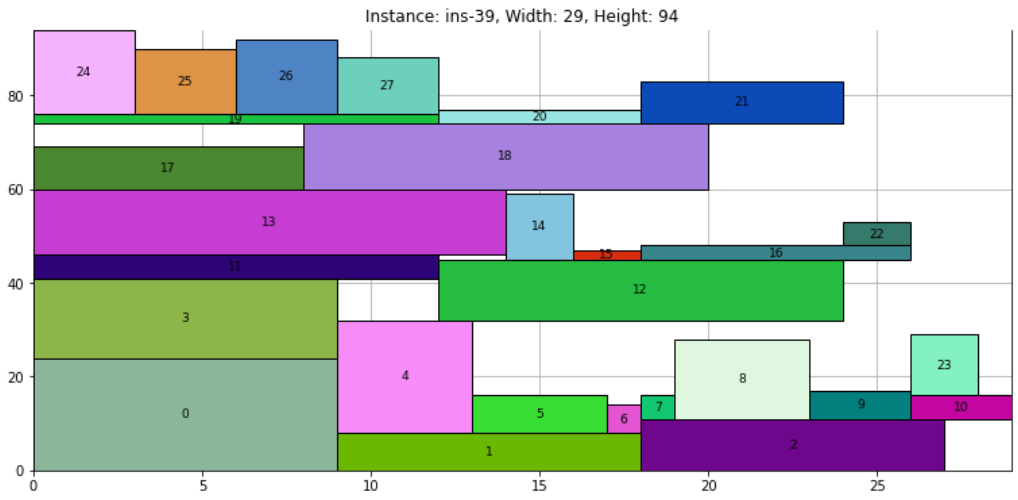
\includegraphics[scale=0.6]{figures/H_UB.png}
  \caption{Image describing the way in which $H_{UB}$ is computed}
  \label{img:H_UB}
\end{figure}
\noindent
Known $H_{LB}$ and $H_{UB}$, the \textit{bisection method} will be used, so the height of the first attempt will be $$H_{{attempt}_{0}} = \lfloor \frac{H_{LB} + H_{UB}}{2} \rfloor$$ and if an assignment for the variables is found, then the new attempted height will be $$H_{{attempt}_{1}} = \lfloor \frac{H_{LB} + H_{{attempt}_{0}}}{2} \rfloor$$, otherwise (in case of failure) it will be $$H_{{attempt}_{1}} = \lfloor \frac{H_{{attempt}_{0}} + H_{UB}}{2} \rfloor$$
In case of rotations it is sufficient to use ${H_{UB}}_{rotation}$ instead of $H_{UB}$.
\newline
Instead of using the bisection method we could have started from the actual lower bound $H_{LB}$ and then increment it up to reaching the upper bound, but this is a good method just if we use the strong hypothesis that the given instances can be placed with a height near to $H_{LB}$.

\section{Encoding}
We've chosen the order encoding to represent natural numbers: in this way we have a direct and easy way to convert numbers from the original to the SAT representation (and viceversa), also simplifying the comparison between numbers.
\newline
An example of order encoding having 4 as the biggest representable natural number:
\begin{align*}
0 \rightarrow 1 1 1 1 \rightarrow& enc_0 = TTTT \\
1 \rightarrow 0 1 1 1 \rightarrow& enc_1 = FTTT \\
2 \rightarrow 0 0 1 1 \rightarrow& enc_2 = FFTT \\
3 \rightarrow 0 0 0 1 \rightarrow& enc_3 =  FFFT \\
4 \rightarrow 0 0 0 0 \rightarrow& enc_4 = FFFF
\end{align*}
\newline
Using this encoding it is easy to see that the encoding of a natural number $n \in [0, n_{max}]$ is $$[ \space \underbrace{F..F}_\text{n} \space \underbrace{T..T}_\text{$n_{max}$-n}]$$ 
\newline
Using the 0-based indexing for the elements of the encoding $enc_a$ of a natural number $a$, we have that 
$$enc_{a,i} \rightarrow enc_{a,i+1}, \qquad i \in \{0,n_{max}-2\}$$
\newline
rewritten as a pure CNF clause:
$$\neg enc_{a,i} \vee enc_{a,i+1}, \qquad i \in \{0,n_{max}-2\}$$
\newline
It is also worth noticing that 
$$enc_{a,j} \Leftrightarrow a \leq j, \qquad j \in \{ 0,n_{max}-1\}$$
\newline
For each rectangle $r_{i}$, the length of the encoding of the $x$ coordinate of the i-th rectangle is 
$$ | enc_{x_{i}} | = W $$
And the length of the encoding of the $y$ coordinate of the i-th rectangle is
$$ | enc_{y_{i}} | = H $$
And to the describe the relative position of the rectangles in the strip we add two kinds of variables: 
\begin{itemize}
\item the left-right $lr_{i,j}$ which is true if $r_i$ is at the left of $r_j$ (and therefore $r_j$ is at the right of $r_i$)
\item the up-down $ud_{i,j}$ which is true if $r_i$ is above $r_j$ (and therefore $r_j$ is below $r_i$)
\end{itemize}
\section{Constraints}
We should take into account that $\textbf{all}$ the whole rectangle and not just the left-bottom corner must fit into the width $W$ and height $H$ of the strip, therefore the following constraints must be satisfied (for each rectangle $r_i$):
$$enc_{x_{i},W-width_i} \wedge ... \wedge enc_{x_{i},W-1}$$
$$enc_{y_{i},H-height_i} \wedge ... \wedge enc_{y_{i},H-1}$$
Then we add the order encoding constraint described in the previous section (for each rectangle $r_i$):
$$\neg enc_{x_i,j} \vee enc_{x_i,j+1} \qquad j \in \{0,..,W-2\}$$
$$\neg enc_{y_i,k} \vee enc_{y_i,k+1} \qquad k \in \{0,..,H-2\}$$
Finally, we have the $\textbf{no-overlap}$ constraints:
\newline
Every rectangle has a relative position w.r.t. another, so (for each rectangle $r_i$,$r_j$ with $i < j$ and $i,j \in \{0,N-1\}$): 
\begin{equation}\label{satformula:relativeposition}
    lr_{i,j} \vee lr_{j,i} \vee ud_{i,j} \vee ud_{j,i}
\end{equation}
We should now chain the meaning of the relative position variables with all the other variables and to do that we can think about that, as an example, if a rectangle is at the left of another, the left rectangle left-bottom corner has a distance from the bottom-left corner of the right rectangle that is at least equal to the width of the left rectangle (we can then extend this reasoning to the up-down positioning)
\begin{equation}\label{satformula:1}
    lr_{i,j} \Rightarrow x_i + width_i \leq x_j
\end{equation}
\begin{equation}\label{satformula:2}
    lr_{j,i} \Rightarrow x_j + width_j \leq x_i
\end{equation}
\begin{equation}\label{satformula:3}
    ud_{i,j} \Rightarrow y_i + height_i \leq y_j
\end{equation}
\begin{equation}\label{satformula:4}
    ud_{j,i} \Rightarrow y_j + height_j \leq y_i
\end{equation}
\newline
\begin{bluebox}
\subsection{Encoding of inequalities in SAT}
if we have an inequality of the form 
$$x + c \leq y$$
where $c \in \{ 0..n_{max}\}$ and so that $|enc_{x}| = |enc_{y}|=n_{max}$, then 
$$x \leq z, \qquad z \in  \{ n_{max}-c, .., n_{max}\} $$
$$y \geq t, \qquad t \in  \{0, ..,c\}$$ 
which can be rewritten as 
$$x \leq z, \qquad z \in  \{ n_{max}-c, .., n_{max}\} $$
$$\neg (y \leq k), \qquad k \in \{0, .., c-1\}$$
$$(y \leq c + s) \rightarrow  (x \leq s), \qquad s \in \{0, .., n_{max} -c- 1\}$$

The formulas above are rewritable as literals, each one corresponding to a simple inequality:

$$enc_{x,z} \qquad z \in  \{ n_{max}-c, .., n_{max}-1\}$$
$$\neg enc_{y,t} \qquad t \in \{0, .., c-1\}$$
$$enc_{y,c+s} \rightarrow enc_{x,s} \qquad s \in \{ 0,.., n_{max}-c-1\}$$ 
which can be rewritten as 
$$enc_{x,z} \qquad z \in  \{ n_{max}-c, .., n_{max}-1\}$$
$$\neg enc_{y,t} \qquad t \in \{0, .., c-1\}$$
$$\neg enc_{y,c+s} \vee enc_{x,s} \qquad s \in \{ 0,.., n_{max}-c-1\}$$
\end{bluebox}

The inequalities are therefore transformed in the following formulas:
\begin{itemize}
    \item Formula \ref{satformula:1} becomes
        \begin{equation}\label{satformula:1_mod}
        \begin{aligned}
            &lr_{i,j} \rightarrow {enc}_{x_{i},z}  \qquad z \in \{W-{width}_i,..,W-1 \}
            \\
            &lr_{i,j} \rightarrow \neg {enc}_{x_{j},t} \qquad t \in \{ 0,.., {width}_i -1\}
            \\
            &lr_{i,j} \rightarrow (\neg {enc}_{x_{j},{width}_i+s} \vee {enc}_{x_{i},s}) \qquad s \in \{ 0,.., W-{width}_i-1\}
        \end{aligned}
        \end{equation}

    \item Formula \ref{satformula:2} becomes
        \begin{equation}\label{satformula:2_mod}
        \begin{aligned}
            &lr_{j,i} \rightarrow {enc}_{x_{j},z}  \qquad z \in \{W-{width}_j,..,W-1 \}
            \\
            &lr_{j,i} \rightarrow \neg {enc}_{x_{i},t} \qquad t \in \{ 0,.., {width}_j -1\}
            \\
            &lr_{j,i} \rightarrow (\neg {enc}_{x_{i},{width}_j+s} \vee {enc}_{x_{j},s}) \qquad s \in \{ 0,.., W-{width}_j-1\}
        \end{aligned}
        \end{equation}

    \item Formula \ref{satformula:3} becomes
        \begin{equation}\label{satformula:3_mod}
        \begin{aligned}
            &ud_{i,j} \rightarrow {enc}_{y_{i},z} \qquad z \in \{ H-{height}_i,..,H-1 \}
            \\
            &ud_{i,j} \rightarrow \neg{enc}_{y_{j},t} \qquad t \in \{ 0,.., {height}_i -1\}
            \\
            &ud_{i,j} \rightarrow (\neg {enc}_{y_{j},height_{i}+s} \vee enc_{y_{i},s}) \qquad s \in \{ 0, ..,H-height_i-1\}
        \end{aligned}
        \end{equation}

    \item Formula \ref{satformula:4} becomes
        \begin{equation}\label{satformula:4_mod}
        \begin{aligned}
            &ud_{j,i} \rightarrow {enc}_{y_{j},z} \qquad z \in \{ H-{height}_j,..,H-1 \}
            \\
            &ud_{j,i} \rightarrow \neg{enc}_{y_{i},t} \qquad t \in \{ 0,.., {height}_j -1\}
            \\
            &ud_{j,i} \rightarrow (\neg {enc}_{y_{i},height_{j}+s} \vee enc_{y_{j},s}) \qquad s \in \{ 0,.., H-height_j-1\}
        \end{aligned}
        \end{equation}
\end{itemize}
\noindent
The first formula of each term can be avoided because the right-hand side of that implication is already made true by the first described constraint, therefore we finally obtain 
\begin{itemize}
    \item Formula \ref{satformula:1_mod} becomes
        \begin{equation}
        \begin{aligned}\label{satformula:1final}
            &\neg lr_{i,j} \vee \neg {enc}_{x_{j},t} \qquad t \in \{ 0,.., {width}_i -1\} \\
            &\neg lr_{i,j} \vee \neg {enc}_{x_{j},{width}_i+s} \vee {enc}_{x_{i},s} \qquad s \in \{ 0,.., W-{width}_i-1\}
        \end{aligned}
        \end{equation}
    \item Formula \ref{satformula:2_mod} becomes
        \begin{equation}
        \begin{aligned}\label{satformula:2final}
            &\neg lr_{j,i} \vee \neg {enc}_{x_{i},t} \qquad t \in \{ 0,.., {width}_j -1\} \\
            &\neg lr_{j,i} \vee \neg {enc}_{x_{i},{width}_j+s} \vee {enc}_{x_{j},s} \qquad s \in \{ 0,.., W-{width}_j-1\}
        \end{aligned}
        \end{equation}

    \item Formula \ref{satformula:3_mod} becomes
        \begin{equation}
        \begin{aligned}\label{satformula:3final}
            & \neg ud_{i,j} \vee \neg{enc}_{y_{j},t} \qquad t \in \{ 0,.., {height}_i -1\} \\
            &\neg ud_{i,j} \vee \neg {enc}_{y_{j},height_{i}+s} \vee enc_{y_{i},s} \qquad s \in \{ 0,.., H-height_i-1\}
        \end{aligned}
        \end{equation}
        
    \item Formula \ref{satformula:4_mod} becomes
    \begin{equation}
    \begin{aligned}\label{satformula:4final}
        &\neg ud_{j,i} \vee \neg{enc}_{y_{i},t} \qquad t \in \{ 0,.., {height}_j -1\} \\
        &\neg ud_{j,i} \vee \neg {enc}_{y_{i},height_{j}+s} \vee enc_{y_{j},s} \qquad s \in \{ 0,.., H-height_j-1\}
    \end{aligned}
    \end{equation}
    
\end{itemize}

\newpage

\section{Symmetry Breaking Constraints}
    In order to make the computation faster it is necessary to prune the search space reducing the number of clauses and literals involved (contrarily to CP, where adding constraints makes the detection of unfeasible solutions faster).
    \newline
    We've applied 3 kinds of Symmetry Breaking Constraints:
\subsection{Large Rectangles (LR) Symmetry Breaking}
    If the sum of two rectangles widths is bigger than the width of the strip (i.e. ${width}_i$ + ${width}_j$>W) we can assume that they can't be placed one on the left or right side of the other and we can delete some of the constraints:
    \newline
    Formula \ref{satformula:relativeposition} is rewritten as 
    \begin{equation*}
         \cancel{lr_{i,j}} \vee \cancel{lr_{j,i}} \vee ud_{i,j} \vee ud_{j,i}
    \end{equation*}

    \begin{itemize}
        \item Formula \ref{satformula:1final} is deleted
            \begin{equation*}
            \cancel{
            \begin{aligned}
                &\neg lr_{i,j} \vee \neg {enc}_{x_{j},t} \qquad t \in \{ 0,.., {width}_i -1\}
                \\
                &\neg lr_{i,j} \vee \neg {enc}_{x_{j},{width}_i+s} \vee {enc}_{x_{i},s} \qquad s \in \{ 0,.., W-{width}_i-1\}
            \end{aligned}
            }
            \end{equation*}
        \item Formula \ref{satformula:2final} is deleted
            \begin{equation*}
            \cancel{
            \begin{aligned}
            &\neg lr_{j,i} \vee \neg {enc}_{x_{i},t} \qquad t \in \{ 0,.., {width}_j -1\}
            \\
            &\neg lr_{j,i} \vee \neg {enc}_{x_{i},{width}_j+s} \vee {enc}_{x_{j},s} \qquad s \in \{ 0,.., W-{width}_j-1\}
            \end{aligned}
            }
            \end{equation*}
        
        \item Formula \ref{satformula:3final} is kept
            \begin{equation*}
            \begin{aligned}
                &\neg ud_{i,j} \vee \neg{enc}_{y_{j},t} \qquad t \in \{ 0, {height}_i -1\} \\
                &\neg ud_{i,j} \vee \neg {enc}_{y_{j},height_{i}+s} \vee enc_{y_{i},s} \qquad s \in \{ 0, H-height_i-1\}
            \end{aligned}
            \end{equation*}
    
        \item Formula \ref{satformula:4final} is kept
            \begin{equation*}
            \begin{aligned}
            &\neg ud_{j,i} \vee \neg{enc}_{y_{i},t} \qquad t \in \{ 0,.., {height}_j -1\}
            \\
            &\neg ud_{j,i} \vee \neg {enc}_{y_{i},height_{j}+s} \vee enc_{y_{j},s} \qquad s \in \{ 0,.., H-height_j-1\}
            \end{aligned}
            \end{equation*}
    \end{itemize}
    We can also apply the same reasoning to the height, because if ${height}_i$ + ${height}_j$>H we can assume that those rectangles can't be placed one above or under the other and we can delete these constraints:
    \newline
    Formula \ref{satformula:relativeposition} is rewritten as
    \begin{equation*}
        lr_{i,j} \vee lr_{j,i} \vee \cancel{ud_{i,j}} \vee \cancel{ud_{j,i}}
    \end{equation*}
    \begin{itemize}
        \item Formula \ref{satformula:1final} is kept
            \begin{equation*}
            \begin{aligned}
                &\neg lr_{i,j} \vee \neg {enc}_{x_{j},t} \qquad t \in \{ 0,.., {width}_i -1\}
                \\
                &\neg lr_{i,j} \vee \neg {enc}_{x_{j},{width}_i+s} \vee {enc}_{x_{i},s} \qquad s \in \{ 0,.., W-{width}_i-1\}
            \end{aligned}
            \end{equation*}
        \item Formula \ref{satformula:2final} is kept
            \begin{equation*}
            \begin{aligned}
                &\neg lr_{j,i} \vee \neg {enc}_{x_{i},t} \qquad t \in \{ 0,.., {width}_j -1\} \\
                &\neg lr_{j,i} \vee \neg {enc}_{x_{i},{width}_j+s} \vee {enc}_{x_{j},s} \qquad s \in \{ 0,.., W-{width}_j-1\}
            \end{aligned}
            \end{equation*}
    
        \item Formula \ref{satformula:3final} is deleted
            \begin{equation*}
            \cancel{
            \begin{aligned}
                &\neg ud_{i,j} \vee \neg{enc}_{y_{j},t} \qquad t \in \{ 0, {height}_i -1\}
                \\
                &\neg ud_{i,j} \vee \neg {enc}_{y_{j},height_{i}+s} \vee enc_{y_{i},s} \qquad s \in \{ 0, H-height_i-1\}
            \end{aligned}
            }
            \end{equation*}
    
       \item Formula \ref{satformula:4final} is deleted
            \begin{equation*}
            \cancel{
            \begin{aligned}
                &\neg ud_{j,i} \vee \neg{enc}_{y_{i},t} \qquad t \in \{ 0,.., {height}_j -1\}
                \\
                &\neg ud_{j,i} \vee \neg {enc}_{y_{i},height_{j}+s} \vee enc_{y_{j},s} \qquad s \in \{ 0,.., H-height_j-1\}
            \end{aligned}
            }
            \end{equation*}
            \end{itemize}


\subsection{Same Sized Rectangles (SR) Symmetry Breaking}
If two rectangles are such that $width_i = width_j$ and $height_i = height_j$ we can choose to have rectangle $i$ left-under $j$:
\newline
Formula \ref{satformula:relativeposition} is rewritten as
\begin{equation*}
    lr_{i,j} \vee \cancel{lr_{j,i}} \vee ud_{i,j} \vee ud_{j,i}
\end{equation*}
%TODO delete formulas in point 2 
\begin{itemize}
    \item Formula \ref{satformula:1final} is kept
        \begin{equation*}
        \begin{aligned}
        &\neg lr_{i,j} \vee \neg {enc}_{x_{j},t} \qquad t \in \{ 0,.., {width}_i -1\}
        \\
        &\neg lr_{i,j} \vee \neg {enc}_{x_{j},{width}_i+s} \vee {enc}_{x_{i},s} \qquad s \in \{ 0,.., W-{width}_i-1\}
        \end{aligned}
        \end{equation*}
    \item Formula \ref{satformula:2final} is deleted
        \begin{equation*}
        \cancel{
        \begin{aligned}
            &\neg lr_{j,i} \vee \neg {enc}_{x_{i},t} \qquad t \in \{ 0,.., {width}_j -1\}
            \\
            &\neg lr_{j,i} \vee \neg {enc}_{x_{i},{width}_j+s} \vee {enc}_{x_{j},s} \qquad s \in \{ 0,.., W-{width}_j-1\}
        \end{aligned}
        }
        \end{equation*}
    \item Formula \ref{satformula:3final} is kept
        \begin{equation*}
        \begin{aligned}
        &\neg ud_{i,j} \vee \neg{enc}_{y_{j},t} \qquad t \in \{ 0,.., {height}_i -1\}
        \\
        &\neg ud_{i,j} \vee \neg {enc}_{y_{j},height_{i}+s} \vee enc_{y_{i},s} \qquad s \in \{ 0,.., H-height_i-1\}
        \end{aligned}
        \end{equation*}
    \item Formula \ref{satformula:4final} is kept
        \begin{equation*}
        \begin{aligned}
        &\neg ud_{j,i} \vee \neg{enc}_{y_{i},t} \qquad t \in \{ 0,.., {height}_j -1\}
        \\
        &\neg ud_{j,i} \vee \neg {enc}_{y_{i},height_{j}+s} \vee enc_{y_{j},s} \qquad s \in \{ 0,.., H-height_j-1\}
        \end{aligned}
        \end{equation*}
\end{itemize}
% this formula is added:
Adding just a new formula:
$$ud_{i,j} \rightarrow {lr}_{j,i}$$ rewritable as $$\neg ud_{i,j} \vee {lr}_{j,i}$$


\subsection{Largest Sized Rectangle (LS) Symmetry Breaking} 

We can also assume to have the biggest rectangle (in terms of area) $largest$ placed in the left bottom half of the rectangle. This makes it possible to restrict the domain:
$$enc_{x_{largest},i}, \qquad i \in \{ \lfloor \frac{W-width_{largest}}{2} \rfloor, W-1 \}$$
$$enc_{y_{largest},j}, \qquad j \in \{ \lfloor \frac{H-height_{largest}}{2} \rfloor, H-1 \}$$
And delete some overlapping constraints:
\newline
Formula \ref{satformula:relativeposition} is rewritten as

\begin{equation*}
    \cancel{lr_{i,largest}} \vee lr_{largest,i} \vee \cancel{ud_{i,largest}} \vee ud_{largest,i}
\end{equation*}

\begin{itemize}
    \item Formula \ref{satformula:1final} is deleted
        \begin{equation*}
            \cancel{
        \begin{aligned}
            &\neg lr_{i,largest} \vee \neg {enc}_{x_{largest},t} \qquad t \in \{ 0,.., {width}_i -1\}
            \\
            &\neg lr_{i,largest} \vee \neg {enc}_{x_{largest},{width}_i+s} \vee {enc}_{x_{i},s} \qquad s \in \{ 0,.., W-{width}_i-1\}
        \end{aligned}
        }
        \end{equation*}
    \item Formula \ref{satformula:2final} is kept
        \begin{equation*}
        \begin{aligned}
            &\neg lr_{largest,i} \vee \neg {enc}_{x_{i},t} \qquad t \in \{ 0,.., {width}_largest -1\}
            \\
            &\neg lr_{largest,i} \vee \neg {enc}_{x_{i},{width}_{largest}+s} \vee {enc}_{x_{largest},s} \qquad s \in \{ 0,.., W-{width}_{largest}-1\}
        \end{aligned}
        \end{equation*}

%this 3.
    \item Formula \ref{satformula:3final} is kept
        \begin{equation*}
        \cancel{
        \begin{aligned}
            &\neg ud_{i,largest} \vee \neg{enc}_{y_{largest},t} \qquad t \in \{ 0,.., {height}_i -1\}
            \\
            &\neg ud_{i,largest} \vee \neg {enc}_{y_{largest},height_{i}+s} \vee enc_{y_{i},s} \qquad s \in \{ 0,.., H-height_i-1\}
        \end{aligned}
        }
        \end{equation*}

    \item Formula \ref{satformula:4final} is kept
        \begin{equation*}
        \begin{aligned}
            &\neg ud_{largest,i} \vee \neg{enc}_{y_{i},t} \qquad t \in \{ 0,.., {height}_{largest} -1\}
            \\
            &\neg ud_{largest,i} \vee \neg {enc}_{y_{i},height_{largest}+s} \vee enc_{y_{largest},s} \qquad s \in \{ 0,.., H-height_{largest}-1\}
        \end{aligned}
        \end{equation*}
\end{itemize}

\section{A variant: rotations}
We've introduced a new variable $r$ for each instance, it is True if the rectangle is rotated, False if it is not. For each of the rectangles, if the height (without rotations) is bigger than the dimension of the whole container, the rotation of that same rectangle is avoided 
\newline
Therefore, we've rewritten the formulas (0-4) in the following way, considering that if a rectangle is rotated, its height and width are inverted:
\begin{itemize}
    \item Formula \ref{satformula:1final} is rewritten as
        \begin{equation*}
        \begin{aligned}
        &\neg R_i \rightarrow (\neg lr_{i,j} \vee \neg {enc}_{x_{j},t}) \qquad t \in \{ 0,.., {width}_i -1\}
        \\
        &\neg R_i \rightarrow (\neg lr_{i,j} \vee \neg {enc}_{x_{j},{width}_i+s} \vee {enc}_{x_{i},s}) \qquad s \in \{ 0,.., W-{width}_i-1\}
        \\
        &R_i \rightarrow (\neg lr_{i,j} \vee \neg {enc}_{x_{j},t}) \qquad t \in \{ 0,.., {height}_i -1\}
        \\
        &R_i \rightarrow (\neg lr_{i,j} \vee \neg {enc}_{x_{j},{height}_i+s} \vee {enc}_{x_{i},s}) \qquad s \in \{ 0,.., W-{height}_i-1\}
        \end{aligned}
        \end{equation*}

    \item Formula \ref{satformula:2final} is rewritten as
        \begin{equation*}
        \begin{aligned}
        &\neg R_j \rightarrow (\neg lr_{j,i} \vee \neg {enc}_{x_{i},t}) \qquad t \in \{ 0,.., {width}_j -1\}
        \\
        &\neg R_j \rightarrow (\neg lr_{j,i} \vee \neg {enc}_{x_{i},{width}_j+s} \vee {enc}_{x_{j},s}) \qquad s \in \{ 0,.., W-{width}_j-1\}
        \\
        &R_j \rightarrow (\neg lr_{j,i} \vee \neg {enc}_{x_{i},t}) \qquad t \in \{ 0,.., {height}_j -1\}
        \\
        &R_j \rightarrow (\neg lr_{j,i} \vee \neg {enc}_{x_{i},{height}_j+s} \vee {enc}_{x_{j},s}) \qquad s \in \{ 0,.., W-{height}_j-1\}
        \end{aligned}
        \end{equation*}

    \item Formula \ref{satformula:3final} is rewritten as
        \begin{equation*}
        \begin{aligned}
        &\neg R_i \rightarrow (\neg ud_{i,j} \vee \neg{enc}_{y_{j},t}) \qquad t \in \{ 0,.., {height}_i -1\}
        \\
        &\neg R_i \rightarrow (\neg ud_{i,j} \vee \neg {enc}_{y_{j},height_{i}+s} \vee enc_{y_{i},s}) \qquad s \in \{ 0,.., H-height_i-1\}
        \\
        &R_i \rightarrow (\neg ud_{i,j} \vee \neg{enc}_{y_{j},t}) \qquad t \in \{ 0,.., {width}_i -1\}
        \\
        &R_i \rightarrow (\neg ud_{i,j} \vee \neg {enc}_{y_{j},width_{i}+s} \vee enc_{y_{i},s}) \qquad s \in \{ 0,.., H-width_i-1\}
        \end{aligned}
        \end{equation*}

    \item Formula \ref{satformula:4final} is rewritten as
        \begin{equation*}
        \begin{aligned}
        &\neg R_j \rightarrow (\neg ud_{j,i} \vee \neg{enc}_{y_{i},t}) \qquad t \in \{ 0,.., {height}_j -1\}
        \\
        &\neg R_j \rightarrow (\neg ud_{j,i} \vee \neg {enc}_{y_{i},height_{j}+s} \vee enc_{y_{j},s}) \qquad s \in \{ 0,.., H-height_j-1\}
        \\
        &R_j \rightarrow (\neg ud_{j,i} \vee \neg{enc}_{y_{i},t}) \qquad t \in \{ 0,.., {width}_j -1\}
        \\
        &R_j \rightarrow (\neg ud_{j,i} \vee \neg {enc}_{y_{i},width_{j}+s} \vee enc_{y_{j},s}) \qquad s \in \{ 0,.., H-width_j-1\}
        \end{aligned}
        \end{equation*}
\end{itemize}
\subsection{Squares Symmetry Breaking}
In the version with rotations, We've added a novel constraint that makes it possible to avoid rotations when the rectangle is actually just a square (in this way we avoid the symmetry obtained simply rotating it). In order to apply this symmetry breaking strategy it is necessary to check if $width_i = height_i$: in that case the additional variable $r_i$ is removed from the constraints.
\section{Results}
All instances have been solved (with at least one of the 4 described SAT constraints encodings) but instance 40. Even if sometimes the Symmetry Breaking techniques improve the solver speed, it may not always be the case, this is due to:
\itemize
	\item \textbf{Thermal throttling}: a common feature for non-industrial PCs
	\item \textbf{CPU job priority scheduling}: the PC is not executing just a single process, but has to manage the timing of many system and app processes, therefore some of the tasks involving the benchmark may have been postponed.
For the last reason in the image are shown both the time taken by the solver alone and the time taken by the solver and the encoding part togheter.
\begin{figure}[H]
  \centering
  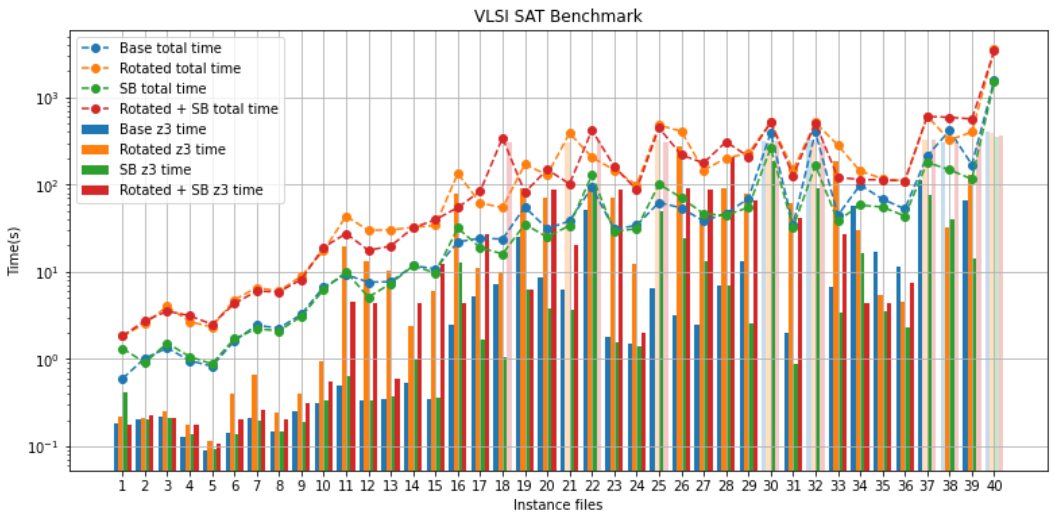
\includegraphics[scale=0.9]{figures/sat_benchmark.png}
  \caption{Image describing the way in which $H_{UB}$ is computed}
  \label{img:H_sat_bench}
\end{figure}
\chapter{SMT}
\chapter{LP}
%\input{mainmatter/chapter-4} % Create file to add

\input{mainmatter/conclusion}

%% Prevent urls running into margins in bibliography
\setcounter{biburlnumpenalty}{7000}
\setcounter{biburllcpenalty}{7000}
\setcounter{biburlucpenalty}{7000}

%% Add bibliography
\printbibliography[heading=bibintoc,title=References]

%% ----------------------------------------------------------------------
%%    Appendix (Letters for chapters)
%% ----------------------------------------------------------------------

\appendix

\chapter{Source Code Example}
%\label{chapter:title}

\emph{Adding source code to your report/thesis is supported with the package {\normalfont\texttt{listings}}. An example can be found below. Files can be added using {\normalfont\texttt{\textbackslash lstinputlisting[language=<language>]\{<filename>\}}}.}

\begin{lstlisting}[language=Python]
"""
ISA Calculator: import the function, specify the height and it will return a
list in the following format: [Temperature,Density,Pressure,Speed of Sound].
Note that there is no check to see if the maximum altitude is reached.
"""

import math
g0 = 9.80665
R = 287.0
layer1 = [0, 288.15, 101325.0]
alt = [0,11000,20000,32000,47000,51000,71000,86000]
a = [-.0065,0,.0010,.0028,0,-.0028,-.0020]

def atmosphere(h):
    for i in range(0,len(alt)-1):
        if h >= alt[i]:
            layer0 = layer1[:]
            layer1[0] = min(h,alt[i+1])
            if a[i] != 0:
                layer1[1] = layer0[1] + a[i]*(layer1[0]-layer0[0])
                layer1[2] = layer0[2] * (layer1[1]/layer0[1])**(-g0/(a[i]*R))
            else:
                layer1[2] = layer0[2]*math.exp((-g0/(R*layer1[1]))*(layer1[0]-layer0[0]))
    return [layer1[1],layer1[2]/(R*layer1[1]),layer1[2],math.sqrt(1.4*R*layer1[1])]
\end{lstlisting}

\chapter{Task Division Example}
%\label{chapter:title}

\emph{If a task division is required, a simple template can be found below for convenience. Feel free to use, adapt or completely remove.}

\begin{table}[htb]
    \setlength\extrarowheight{4pt}
    \centering
    \caption{Distribution of the workload}
    \label{tab:taskdivision}
    \begin{tabularx}{\textwidth}{lXX}
        \toprule
        & Task & Student Name(s) \\
        \midrule
        & Summary & \\
        Chapter 1 & Introduction &  \\
        Chapter 2 &  & \\
        Chapter 3 &  & \\
        Chapter * &  & \\
        Chapter * & Conclusion &  \\
        \midrule
        & Editors & \\
        & CAD and Figures & \\
        & Document Design and Layout & \\
        \bottomrule
    \end{tabularx}
\end{table}

%\input{appendix/appendix-c} % Create file to add

\end{document}
